% !TEX encoding = UTF-8 Unicode
% !TEX root = ..\main.tex
% !TEX spellcheck = en-US
\chapter{Introduction}

\section{Motivation and Background}
The field of embedded systems is growing rapidly based on the evolution in electronics and widespread use of sensors and actuators. From consumer electronics, automobiles, to satellites, embedded systems represent one of the largest segments of the software industry. The automotive domain is going through a major transition where all car manufacturers are working towards the development of self-driving cars. Internet of Things describes the concept of interconnecting the virtual world of computers with the real world of physical artifacts\cite{mattern2010internet}. This leads to a distributed network of devices communicating with other devices as well as humans. Gartner\cite{gartner} have estimated that in 2020, 25 billion connected "things" will be in use. Our society has come to depend on such systems for its day-to-day operation. Embedded systems is forecasted to grow exponentially in the next 10 years\cite{graaf2003embedded}

Software plays an important role in the development of embedded systems\cite{ebert2009embedded}. Embedded software is the primary driving force for implementing different functionalities of today's embedded systems. The software is specialized for one particular type of hardware, and may therefore have hardware specific run-time constraints. As the complexity of embedded system grows, the ability to maintain the required quality of such systems becomes more difficult\cite{ebert2009embedded}. Traditional software development technologies do not take into account the specific needs of embedded systems development\cite{graaf2003embedded}.

Moreover, many companies are forced to think about their time-to-market strategy to keep up with the increased competition. Companies need to decide what kind of shortcuts they will have to take in the development process. Such compromises causes the creation of a financial overhead in the future maintenance activities, usually termed as Technical Debt (TD)\cite{p29-cunningham}. As the amount of TD accumulated in the developed embedded systems grows continuously, companies need to manage the overall debt while keeping the system flexible and extensible. Defects can cause life-threatening situations, delays can create hugs costs, and insufficient productivity can impact an entire company\cite{ebert2009embedded}. Pacemakers are a good example of how embedded software helps millions of person live a better live. Yet between 1990 and 2000, software errors accounted for about 40\% of half million devices recalled\cite{ebert2009embedded}. If the companies could catch software defects earlier in the system design process, their income would be saved. It is necessary for companies to find out how to make decisions so future maintenance and evolution has as low cost as possible. 

According to Gartner\cite{gartner2010}, the cost of dealing with TD threatens to grow to \$1 trillion globally by 2015. That is the double of the amount of TD in 2010. IT management teams must measure the level of TD in their products, and develop a strategy to deal with TD.

%Embedded software is far more complex due to real-time and interface constraints that do not affect IT, application, or desktop software\cite{ebert2009embedded}


\begin{table}[H]
	\centering
	\begin{tabular}{ | l | l | l | l | l |}
	\hline
	\textbf{Category} & \textbf{2013} & \textbf{2014} & \textbf{2015} & \textbf{2020} \\ \hline
	Automotive & 96.0 & 189.6 & 372.3 & 3,511.1 \\ \hline
	Consumer & 1,842.1 & 2,244.5 & 2,874.9 & 13,172.5 \\ \hline
	Generic Business & 395.2 & 479.4 & 623.9 & 5,158.6 \\ \hline
	Vertical Business & 698.7 & 836.5 & 1,009.4 & 3,164.4 \\ \hline
	\textbf{Grand Total} & \textbf{3,032.0} & \textbf{3,750.0} & \textbf{4,880.6} & \textbf{25,006.6} \\
	\hline
	\end{tabular}
	\caption{Internet of Things Units Installed Base by Category\cite{gartner}} \label{tab:table1}
\end{table}


\section{Research Questions}
The main objective of this research is to increase the knowledge of TD by looking at the significant sources, and practices for managing the debt. The reason for this is that embedded systems usually has long lifetime, and it is important to find out how such systems are managed because the architecture and design decisions are usually made long time ago and the decision makers might not be available anymore. 

\textbf{The research questions in this research will be:} 
\begin{itemize}
	\item \textbf{RQ1}: What practices and tools exists for managing technical debt? How are they used?
	\item \textbf{RQ2}: What are the most significant sources of technical debt?
	\item \textbf{RQ3}: When should a technical debt be paid?
	\item \textbf{RQ4}: Who is responsible for deciding whether to incur, or pay off technical debt?
\end{itemize}

\section{Research Method}
The most relevant research methodologies in software engineering are illustrated in Figure \ref{fig:researchProcess}. Throughout this research, the research process illustrated in the model will be used as a basis for the elaboration of how to conduct the research in the upcoming master thesis. 

\begin{figure}[H]
	\centering
	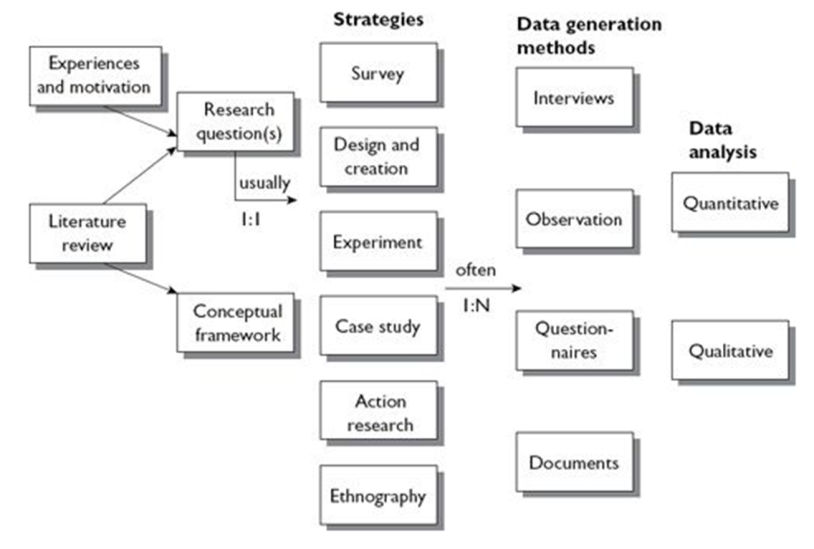
\includegraphics[width=0.8\textwidth]{images/researchStrategies.png}
	\caption{Model of research process\cite{Oates:2006:RIS:1202299}}
	\label{fig:researchProcess}
\end{figure}

To define the research questions, it is necessary to get an overview of the research field by conducting a review of published research within the selected area of study, providing a conceptual framework. Moreover, researchers can use their experiences and motivations. A research strategy is needed to answer the research questions. Oates\cite{Oates:2006:RIS:1202299} presents six different research strategies: survey, design and creation, experiment, case study, action research, and ethnography. A data collection method is needed to produce empirical data or evidence. Furthermore, Oates\cite{Oates:2006:RIS:1202299} presents four different data collection methods: interviews, observations, questionnaire, and documents. Research data can either be quantitative or qualitative. 



\section{Project Structure}
The report is structured into several chapters:
\begin{itemize}
	\item \textbf{Chapter 1} introduces the problem and motivation behind this project along with the search questions.
	\item \textbf{Chapter 2} provides a state-of-art within the field of TD, embedded systems, and software engineering.
	\item \textbf{Chapter 3} presents the research method, and the procedures that was used behind the method.
	\item \textbf{Chapter 4} provides an overview of the results acquired from the research method.
	\item \textbf{Chapter 5} presents a discussion of the relevant topics related to the research questions.
	\item \textbf{Chapter 6} concludes the report and provides some points to future work. 
\end{itemize}

